\documentclass[10pt,b5paper,twoside,openany]{ltjsbook}
% 10pt: フォントサイズ
% b5paper: B5
% twoside: 両面印刷用設定 偶数ページと奇数ページでレイアウトが変化する
% openany: 章変更時に空白ページを挿入しない

% packages
\usepackage[T1]{fontenc}
\usepackage[utf8]{inputenc}
\usepackage[backend=biber, maxnames=100, backref=true]{biblatex}
\usepackage[binary-units = true]{siunitx}
\usepackage{amsmath, amssymb, amsthm}
\usepackage{graphicx}
\usepackage{hyperref}
\usepackage{ascmac}
\usepackage{here}
\usepackage{comment}
\usepackage{listings}
\usepackage{multicol}
\usepackage{wrapfig}
\usepackage{bxpapersize}
\usepackage{biblatex}

% 参考文献追加 + 全ての文献を表示
\nocite{*}
\addbibresource{bibliography.bib}

%= 余白設定(いじらないでください)
%== 横余白
% 137 + 20 + 25 = 182mm
\setlength{\oddsidemargin}{-1truein}        % デフォルトの余白1inchを消す
\setlength{\evensidemargin}{-1truein}       % デフォルトの余白1inchを消す
\setlength{\textwidth}{152truemm}       % テキスト横幅
\setlength{\fullwidth}{\textwidth}      % テキストが柱の線に合うように
\addtolength{\oddsidemargin}{15truemm}  % ノド15mm
\addtolength{\evensidemargin}{15truemm} % 小口15mm
%
%== 縦余白
% 209 + 20 + 20 + 8  = 257mm
\setlength{\topmargin}{-1truein}            % デフォルトの余白1inchを消す
\setlength{\headheight}{0truemm}        % ヘッダ長
\setlength{\textheight}{209truemm}      % テキスト縦幅
\setlength{\headsep}{8truemm}           % ヘッダと本文の間隔
\addtolength{\topmargin}{20truemm}      % 天20mm
%

% ソースコードの設定
\lstset{
  basicstyle={\ttfamily},
  identifierstyle={\small},
  commentstyle={\smallitshape},
  keywordstyle={\small\bfseries},
  ndkeywordstyle={\small},
  stringstyle={\small\ttfamily},
  frame={tb},
  breaklines=true,
  columns=[l]{fullflexible},
  numbers=left,
  xrightmargin=0\zw,
  xleftmargin=3\zw,
  numberstyle={\scriptsize},
  stepnumber=1,
  numbersep=1\zw,
  lineskip=-0.5ex
}

% .aiファイルをpdfファイルとして認識させる
\DeclareGraphicsRule{.ai}{pdf}{.ai}{}

% chapterの余白設定
\makeatletter
\renewcommand{\chapter}{%
  \if@openright\cleardoublepage\else\clearpage\fi
  \global\@topnum\z@
  \secdef\@chapter\@schapter}
\makeatother

% 本文
\begin{document}

% 表紙裏
\thispagestyle{empty}
\mbox{}
\newpage

% 本文
\chapter*{はじめに}
\addcontentsline{toc}{chapter}{はじめに}
みなさんはゲームをやっていますか?
PCでやるゲームと言えば、アクションゲーム、リズムゲーム、RPGなどがありますが、この本で扱うのはいわゆるノベルゲームと呼ばれるタイプのゲームについてです。

例えばみなさんは以下のような経験をしたことはありませんか?
\begin{itemize}
    \item 自宅のWindows機でやっているゲームを出先でもやりたいがMacしか持ってなくてできない……!
    \item Windowsしか対応してないけど宗教上の理由でWindowsが使えない… Vineだと動かないし…
\end{itemize}
こんなときにOSなどのプラットフォームに依存しないような実行環境があったら良いと思いませんか?

プラットフォーム非依存の環境で動作させるとなるとQtやJavaなどのクロスプラットフォームを採用しているソフトやライブラリで開発をすれば可能です。
しかし今までに発売されたソフトの中にはWindowsでしか動かないようなソフトも当然ありますし、それらのソフトに対する答えにはなりえません。

そこでこの本ではOSに依存しない環境で(主にWindows専用ソフトを対象とした)ノベルゲームを実行するためのプラットフォームを作ろうと奮闘した本です。
内容的にはまだまだですが、筆者が本を作ってみたいなどの個人的な都合などもあり、筆を取ることにしました。
本の内容としてはUEFIの基本的な内容から実際にどのように実装したのかまでを(なるべく)詳しく書いてみました。
誤字や誤記、間違いなどもあるかもしれませんが、見つけた時は遠慮なく教えていただけると幸いです。

\tableofcontents
\clearpage

\chapter{UEFIとは}
\begin{wrapfigure}{r}[5pt]{0.3\linewidth}
    \centering
    \includegraphics[scale=0.5]{pic/uefi.ai}
    \caption{EFIとOS、ファームウェアの関係図}
    \label{fig:efi_os_firmware}
\end{wrapfigure}
UEFIはUnified Extensible Firmware Interfaceの略で、OSとプラットフォームファームウェア間を結ぶインターフェースのことを指します。
一言で言うとBIOSの後継のようなものですが、BIOSから機能が大幅に拡張、変更されています。
BIOSでは基本的にOSのロードを行うブートローダーとしての役割がほとんどでしたが、UEFIではそのロードの前段階であらかじめ用意された多くの機能を扱うことができます。
また様々なハードウェア上で動作するように設計されているため、移植が比較的容易であるという利点もあります。
\footnote{もちろんハード依存の処理がある場合はその限りではありません。}

元々はIntelが1998年に開始したIntel Boot Initiativeが元になっており、2000年にEFIの仕様書が始めて作成されました。
\footnote{ただしこれは法的に問題があったため、2002年のバージョンアップからが正式となっています}
現在の最新バージョンは2.8です。

この本では、提供されるランタイム機能を駆使してUEFIアプリ(ノベルゲームの土台)を作成します。
そのUEFIアプリを作るのは別に仕様書を片手に全部1から書くことができますが、普通は開発用のツールが提供されています。
UEFIアプリでは主にEDK2とgnu-efiの2つが有名なツールです。

両者の大きな違いは機能の差です。
gnu-efiはUEFIのランタイムを扱う最低限の機能が提供されており、EDK2はこれに加えてpython、libcなどのより高水準の機能が使えます。
この本ではDocker上で実行することやMakefileを扱う関係からgnu-efiを用いて開発を行っています。

\chapter{環境構築}
この本ではUEFIアプリをDockerを使って開発します。
Dockerを使う理由としてはgnu-efiを使う関係でgccをいれる必要があり、ホスト側に構築すると環境が汚れてしまうという問題があったためです。
\footnote{後述しますがclangで生成することも可能です。この時点では知りませんでした。}
そのためホスト側の環境を汚さないようにするため、コンパイル部分にDockerを使っています。

\section{開発環境}
今回は以下の開発環境で開発を行っています。
\begin{table}[H]
    \centering
    \begin{tabular}{|c|c|}
        \hline
        PC & MacBook Air (13-inch, Early 2015) \\
        CPU & Intel Core i5-5250U @ 1.60GHz \\
        Memory & 8GB \\
        OS & macOS Mojave 10.14.5 \\
        \hline
    \end{tabular}
\end{table}
後述しますが、コンパイルにはdockerを使うのでDockerが動く環境であれば他のOSでも同じように動きます。

使用したソフトは、
\begin{itemize}
    \item Docker Desktop Community Ver. 2.0.0.3 (31259)
    \item QEMU emulator version 4.0.0
\end{itemize}
Docker上で使用したライブラリは、
\begin{itemize}
    \item gcc 8.2.0
    \item curl 7.63.0 (x86\_64)
    \item gnu-efi 3.0.9
\end{itemize}
です。

開発環境を構築する上でのディレクトリ構成も以下に示します。
(efi-storyという名前のディレクトリを想定しています)
{
    \centering
    \begin{verbatim}
        ./efi-story
        |-- Dockerfile
        |-- docker-compose.yml
        +-- src
            |-- Makefile
            |-- main.c
            |-- main.efi
            |-- main.h
            |-- stb_image.h
    \end{verbatim}
}
ディレクトリ直下にDockerfileとdocker-compose.yml、srcディレクトリを配置し、srcディレクトリの下に実際のソースコードなどを置きます。
Dockerを使った開発の流れは、
\begin{enumerate}
    \item ホスト環境でコードを編集する(srcディレクトリ以下)
    \item ルートディレクトリ上でdockerコンテナを実行してコンパイル
    \item コンパイルが完了するとDockerコンテナとの共有ディレクトリ(srcディレクトリ)にファイルが生成される
    \item ホスト上で実行(今回はQEMU)
\end{enumerate} 
のような形で行います。

\section{構築手順}
ここからの手順はDockerをインストールしている前提で話を進めます。
\subsection{Dockerコンテナの作成}
まずはDockerコンテナを作成するところから始めます。

実際のDockerfileを以下に示します。
\begin{lstlisting}[caption=dockerfile,label=dockerfile]
FROM alpine:latest

ENV GNUEFI_VERSION 3.0.9

WORKDIR /var

RUN apk --update add --virtual build-dependences \
        build-base \
        curl \
    && curl -sSL "https://sourceforge.net/projects/gnu-efi/files/gnu-efi-${GNUEFI_VERSION}.tar.bz2/download" -o gnu-efi.tar.bz2 \
    && tar xvf gnu-efi.tar.bz2 \
    && ls \
    && cd gnu-efi-${GNUEFI_VERSION} \
    && make \
    && make install \
    && mkdir /var/gnuefi/ \
    && cd /var/gnuefi

WORKDIR /var/gnuefi
CMD ["make"]
\end{lstlisting}
今回は軽量LinuxディストリビューションであるAlpine Linuxを使っています。

Alpine LinuxはMusl LibcとBusyboxを基にしたLinuxディストリビューションで、非常に軽量であることから数多くのDockerコンテナで採用されています。
\footnote{\url{https://alpinelinux.org/}}
Alpine Linuxではパッケージのインストールにapkと呼ばれるパッケージマネージャを利用します。

コンテナ上ではbuild-baseとcurlをインストールしています。
build-baseは他のディストリビューションでいうbuild-essentialみたいなもので、開発に必要な機能を提供します。
curlはこの下にあるgnu-efiのダウンロードに使用しています。
インストールしているのはこの2つのみですが、build-dependenciesというグループでまとめることで後々消すことになった場合などに一括して消せるようにしています。
\footnote{今のところこれが必要になった場面はありませんが…}

apkで必要なパッケージをインストールした後はgnu-efiのコンパイルを行います。
特に指定する項目などは無いので単純にmake \&\& make installでコンパイル、インストールをしています。

その後の処理はホスト側との共有用のディレクトリを作成しています。
Dockerfile上では共有設定をしていませんが、この後示すdocker-compose上で共有設定を行います。

次にdocker-composeファイルの中身を以下に示します。
\begin{lstlisting}[caption=docker-compose,label=docker-compose]
version: '3'
services:
    uefi-story:
        build: .
        container_name: efi-story
        volumes:
            - ./src:/var/gnuefi
\end{lstlisting}
1つしかコンテナが無いのになんでdocker-compose使っている理由は筆者がDocker単体でボリューム設定をうまく出来なかったからです…。
\footnote{真面目に読んでて分からなかったのでdocker-composeに逃げてしまっていますが、あんまり良くは無い気がするので機会を見て挑戦したいところです。}    
一番最後の行でコンテナ内のディレクトリとホスト側のディレクトリの共有設定を行っています。

これで環境構築は完了です。

\section{実行ファイルの生成}
UEFIアプリの実行ファイルはPE32+形式です。
これはWindows上で使用される実行ファイルの形式であり、本来であればWindows以外の環境(今回はLinux)では生成できません。
そのため、PE32+形式となるように生成ファイルに変更を加える必要があります。
生成ファイルの変更はobjcopyを用いてUEFIアプリケーションとして認識されるように書き換えています。
\footnote{具体的にどうやっているのかは筆者も勉強中です}

生成ファイルの変更する以外に、clang(LLVM)から直接PE32+形式のファイルを生成することも可能です。
その場合は環境を汚さないためDockerも必要なくなります。
\footnote{詳しくは\url{https://dvdhrm.github.io/2019/01/31/goodbye-gnuefi/}参照。夏コミ以降で筆者も試してみるつもりです。}

\section{UEFI in QEMU}
QEMUでUEFIを扱うには、OVMF(Open Virtual Machine Hardware)と呼ばれるファームウェアを用いる必要があります。
OVMFはEDK2の一部として現在は配布されているので
\footnote{\url{https://github.com/tianocore/edk2/tree/master/OvmfPkg}}
そこからダウンロードしますが、ビルドが必要になります。
今回はSourceForgeにあるビルド済のバイナリを用いています。
\footnote{\url{https://sourceforge.net/projects/edk2/files/OVMF/}}
この処理はMakefile上に記載しています(後述)。


3段階に分かれてコマンドを叩くのは面倒なので、Makefileを用いてmakeコマンドのみで実行までできるようにしています。

\chapter{実装項目と詳細}
UEFIアプリ上でノベルゲームを作る上で実装する機能を以下に示します。
\begin{multicols}{2}
    \centering
    \begin{itemize}
        \item ファイル処理
        \begin{itemize}
            \item ファイルボリュームのオープン
            \item ファイルの読み込み
        \end{itemize}
        \item 画像処理
        \begin{itemize}
            \item 透過処理
            \item バッファリング
        \end{itemize}
        \item BGM
        \columnbreak
        \item テキスト
        \begin{itemize}
            \item フォント(TrueTypeなど)
            \item 可変長変数の入力
        \end{itemize}
        \item キー入力
    \end{itemize}
\end{multicols}
この本ではBGM、フォントのTrueType対応を除く部分を実装しました。
ソースコード類はGitHubに上げています。
\footnote{\url{https://github.com/komekome09/efi-story}}
この本の中でソースコードまで載せるのは量が増えすぎてしまうので適宜コードを見ながら読んでください。
以下では実装に使った関数や実装方法などを載せています。

\section{プログラミングをする上でのUEFI}
実装について説明する前にUEFIランタイム(とgnu-efi)を扱う上で気をつけておく(自分が気になった)点を説明します。
\subsection{プロトコルとハンドラ}
一般的なプログラミング言語と同様に、UEFIのプロトコルもメモリ上にある関数へのポインタを経由して関数を呼び出しています。
その関数ポインタや識別するためのGUID、関数を使用するのに必要なデータ構造などをまとめた構造体がプロトコルと呼んでいるものです。
UEFI上ではこのプロトコルを使うためにはそのプロトコルのハンドラを取得し、そこからプロトコルを取得する必要があります。
gnu-efiではLibLocateProtocol関数を使うだけでプロトコルが使用可能な状態にしてくれますが、中身としてはハンドラの取得
\footnote{LocateHandle関数}
、プロトコルの取得
\footnote{HandleProtocol関数}
の2段階でプロトコルを取得しています。

\subsection{uefi\_call\_wrapper}
gnu-efiで関数を呼び出す際は
\begin{lstlisting}[caption=call function with gnu-efi,label=cfgnuefi]
uefi_call_wrapper(GraphicsOutput->Blt, 10, GraphicsOutput, BltBuffer, EfiBltBufferToVideo, 0, 0, 0, 0, DispWidth, DispHeight, DispWidth * sizeof(EFI_GRAPHICS_OUTPUT_BLT_PIXEL));
\end{lstlisting}
のように\verb+uefi_call_wrapper+関数を用いてラッパーとして呼び出します。
この\verb+uefi_call_wrapper+関数はABI(Application Binary Interface)の差異を吸収するためのマクロです。
コンパイルした後に生成されるファイルは機械語として出力されていますが、機械語に変換する際にABIは用いられます。
正確には使用しているデータ構造や処理内容が機械語ではどのように表わせるかを規定したものです。
\footnote{今回はMicrosoft ABIとSysv ABIの差異を吸収するのに用いられています。}
gnu-efiでは\verb+uefi_call_wrapper+マクロを使わないと呼び出せない場合があるので基本的にはこのマクロ経由で呼び出すようにしましょう。
\footnote{たまに忘れてなんで動かないんだこれってなります。}

\section{ファイル処理}
ファイル処理はEFIインターフェースで提供されています。

ファイルの処理には読み込む前にまずファイルが存在するディレクトリボリュームを開く必要があります。
ディレクトリボリュームは\verb+EFI_SIMPLE_FILE_SYSTEM_PROTOCOL+内のOpenVolume関数を用いて開きます。
必要となる部分だけ抜粋して載せます。
\begin{lstlisting}[caption=EFI\_SIMPLE\_FILE\_SYSTEM\_PROTOCOL,label=efi_simple_file_system_protocol]
typedef struct _EFI_SIMPLE_FILE_SYSTEM_PROTOCOL {
    UINT64 Revision;
    EFI_SIMPLE_FILE_SYSTEM_PROTOCOL_OPEN_VOLUME OpenVolume;
} EFI_SIMPLE_FILE_SYSTEM_PROTOCOL
\end{lstlisting}
\begin{lstlisting}[caption=EFI\_FILE\_PROTOCOL,label=efi_file_protocol]
typedef struct _EFI_FILE_PROTOCOL {
    UINT64         Revision;
    EFI_FILE_OPEN     Open;
    EFI_FILE_CLOSE     Close;
    EFI_FILE_DELETE    Delete;
    EFI_FILE_READ     Read;
    EFI_FILE_WRITE     Write;
    ︙
    } EFI_FILE_PROTOCOL;
\end{lstlisting}    
その後\verb+EFI_FILE_PROTOCOL+内のOpen関数でファイルを開き、先に確保したメモリ空間にRead関数を用いてデータを読み込みます。
ファイルサイズがOpenした状態では分からないため、ある程度の大きさのメモリ領域を確保した上で読み込み、その後メモリサイズをリサイズするという処理をしています。
\footnote{書いている途中にGetInfo関数で取れることに気づきました…}

\section{画像処理}
画像処理は表示するだけならEFIインターフェースで可能です。
表示には各ピクセルのRGBデータを得る必要がありますが、画像ファイルが圧縮されている場合などは解凍処理などを実装する必要があります。
また、透過処理(アルファブレンドなど)も実装が必要となります。
ノベルゲームなどでは図\ref{fig:nobel_exp}に示すようにテキストを表示する枠の部分(ピンク色)が背景画像(橙色)に対して透過していることが多々あるため、機能としては必須と考えています。
\begin{figure}[H]
    \centering
    \includegraphics[scale=0.3]{pic/nobel_exp.ai}
    \caption{ノベルゲームの表示例}
    \label{fig:nobel_exp}
\end{figure}

UEFI上での描画には、\verb+EFI_GRAPHICS_OUTPUT_PROTOCOL+というプロトコルを利用します。
\verb+EFI_GRAPHICS_OUTPUT_PROTOCOL+と\verb+EFI_GRAPHICS_OUTPUT_BLT_PIXEL+の構造を使用する部分だけ抜粋したのを以下に示します。
\begin{lstlisting}[caption=EFI\_GRAPHICS\_OUTPUT\_PROTOCOL,label=efi_gop]
typedef struct EFI_GRAPHICS_OUTPUT_PROTCOL {
    ︙
    EFI_GRAPHICS_OUTPUT_PROTOCOL_BLT        Blt;
    EFI_GRAPHICS_OUTPUT_PROTOCOL_MODE       *Mode;
} EFI_GRAPHICS_OUTPUT_PROTOCOL;
\end{lstlisting}
\begin{lstlisting}[caption=EFI\_GRAPHICS\_OUTPUT\_BLT\_PIXEL+,label=efi_gobp]
typedef struct {
    UINT8 Blue;
    UINT8 Green;
    UINT8 Red;
    UINT8 Reserved;
} EFI_GRAPHICS_OUTPUT_BLT_PIXEL;
\end{lstlisting}
このプロトコルには他にも2つの関数(QueryMode関数、SetMode関数)と1つの変数(Mode)があり、その中でも描画はBlt関数で行います。
具体的な描画プロセスは、1ピクセル毎のデータを表現する\verb+EFI_GRAPHICS_OUTPUT_BLT_PIXEL+構造体に代入し、それをフレームバッファーに描きこむことで描画します。
このフレームバッファーに描画する関数がBlt関数です。
\footnote{フレームバッファーに描画するだけでなく、読み込むことも出来ます。}
フレームバッファーにはアドレスを取得して直接書き込む方法もありますが、今回はダブルバッファリング(描画メモリと別のメモリ上との)を行うためBlt関数を使用しています。

画像ファイルは最初にRGBの生データに変換してから\verb+EFI_GRAPHICS_OUTPUT_BLT_PIXEL+構造体に代入します。
生データへの変換はnothings氏が作成したstbと呼ばれる単一ファイルから構成されるライブラリを利用しました。
\footnote{\url{https://github.com/nothings/stb} ライセンスはパブリックドメインです。}
このライブラリはlibcを利用しているため、libc関連の処理は全て置き換える必要があります。
変換した関数と置き換え後の関数の一覧を以下に示します。
\begin{table}[H]
    \centering
    \begin{tabular}{|c|c|}
        \hline
        置き換え前 & 置き換え後 \\
        \hline
        malloc & AllocatePool \\
        realloc & ReallocatePool \\
        free & FreePool \\
        memcpy & CopyMem \\
        memset & ZeroMem or SetMem \\
        \hline
    \end{tabular}
    \label{tb:function}
\end{table}
ここで挙げた置き換え後の関数は全部を網羅していませんが、最低限これだけの置き換えを行うことで動作しています。
また、全てUEFIのランタイム関数ではなくgnu-efi内で定義されている関数です。

処理の流れとしては以下のようになります。
\begin{itemize}
    \item ファイルの読み込み
    \item ライブラリを利用して別のメモリ領域に画像のRGBデータを読み込む
    \item フレームバッファに書き込み
    \item ディスプレイに描画
\end{itemize}
この処理を繰り返すことで描画を行います。

\section{BGM}
BGMに関してはUEFIが提供しているインターフェースに音楽などの再生機能が無いため、ドライバ経由でアクセスするなどの手段を自力で実装する必要があります。
実装方法としてはPCスピーカーを使う方法がもっとも単純ですが、いわゆるビープ音しか鳴らせないためHDA(High Difinition Audio)インターフェースに対応することでより高音質なデータを扱うことができます。
この本ではBGMに関しては述べません。

\section{テキスト}
インターフェース自体にも文字の出力関数は用意されていますが、画像で塗り潰してしまうため見えなくなるというのと、図\ref{fig:defaultfont}のように見栄えが非常に悪くなるという問題があります。
\begin{figure}[H]
    \centering
    \begin{tabular}{c}
        \begin{minipage}{0.5\hsize}
            \centering
            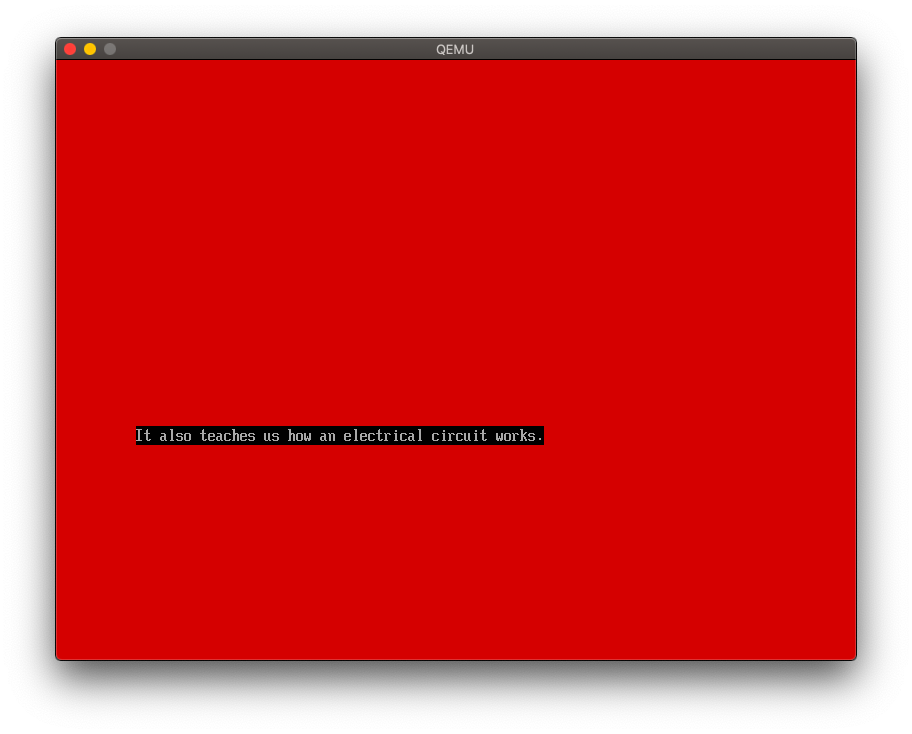
\includegraphics[scale=0.22]{pic/defaultfont.png}
            \caption{標準インターフェースでの文字の表示例}
            \label{fig:defaultfont}
        \end{minipage}
        \begin{minipage}{0.5\hsize}
            \centering
            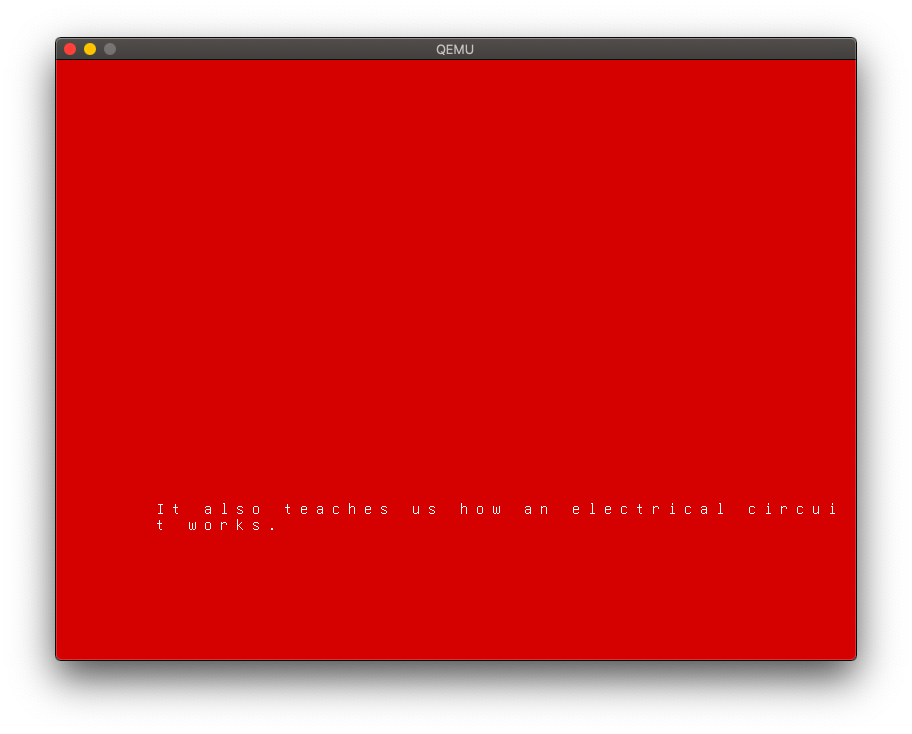
\includegraphics[scale=0.22]{pic/screenshot.png}
            \caption{透過処理を施したビットマップフォントでの文字の表示例}
            \label{fig:bitmapfont}
        \end{minipage}
    \end{tabular}  
\end{figure}
そのため、フォントを画像として表示することで各種問題を回避しています(図\ref{fig:bitmapfont})。
今回はGNU Unifontのビットマップ画像を用いたフォント表示を実装することにしました。
ビットマップフォントなので見た目はよろしくありませんが、背景色で透過できるためより自然な見た目になります。
将来的にはTrueTypeフォントを扱えるようにすることでより綺麗にフォントが表示することを考えています。

今回フォントの表示にはビットマップフォントを用いるので画像処理が出来ればフォント処理も同様に可能です。
ただしそのまま表示すると下の図のようにフォントの部分だけ背景が黒色になってしまうので、透過処理が必要になります。
\begin{figure}[H]
    \centering
    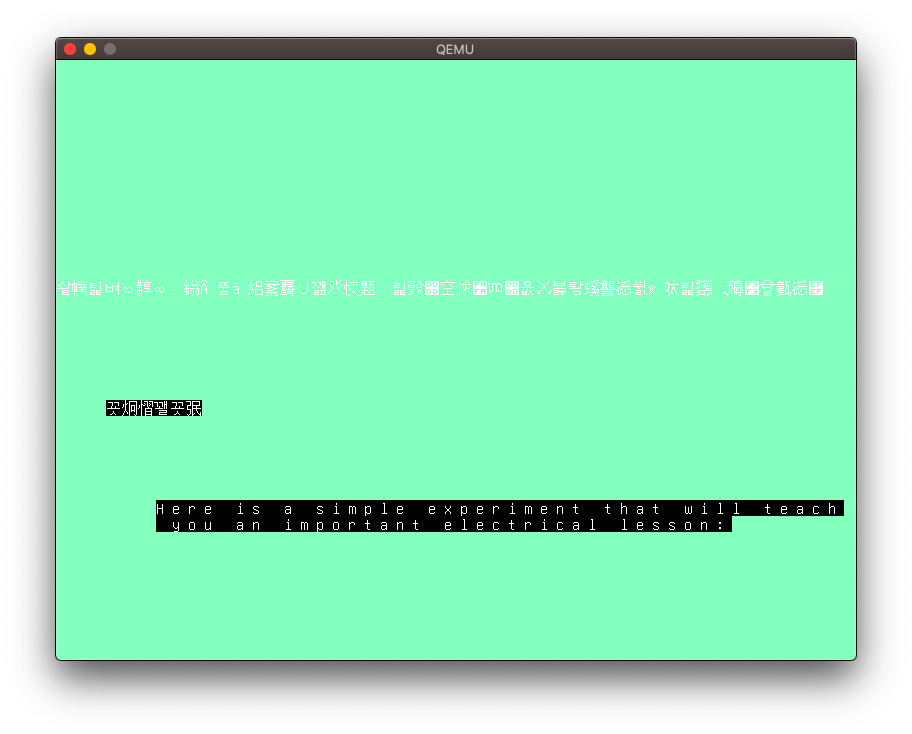
\includegraphics[scale=0.25]{pic/font_with_backblack.png}
    \caption{フォントの背景色を透過しなかった場合の結果}
    \label{fig:font_with_backblack}
\end{figure}
透過処理はRGBが指定した値以下であれば書き換えずに次のピクセルに移動するという非常に単純な処理です。

与えられた文字から画像データに変換するのにはUnicodeの符号位置をビットマップ上の位置に変換することで表示します。
UEFIでは標準で2バイトUnicodeを採用しているため、そこから上位ビットと下位ビットを抜き出すことで横軸上位ビット、縦軸下位ビットの組み合わせに落とし込むことが可能です。

\section{キー処理}
キー入力はReadKeyStroke関数を用いることで取得することが可能です。
ReadKeyStroke関数を実行すると\verb+EFI_INPUT_KEY+構造体に関数実行時点での入力キーが代入されます。
\verb+EFI_INPUT_KEY+構造体は以下のように定義されます。
\begin{lstlisting}[caption=EFI\_INPUT\_KEY,label=efi_input_key]
typedef struct {
    unsigned short ScanCode;
    unsigned short UnicodeChar;
} EFI_INPUT_KEY;
\end{lstlisting}
ScanCodeはUnicodeで表現できない文字が入力された場合に格納される変数です。
例えばEscキーが入力されるとScanCodeには0x17(23)が代入されます。
UTF-16で表現できる場合は0が代入されます。

UnicodeCharはScanCodeとは逆にUnicodeで表現できる文字が入力された場合に対応する文字を代入します。
Unicodeで表現できない文字の場合は0を代入します。

\chapter{あとがき}
hogehogehogeblahblahblah
\newpage

\thispagestyle{empty}
\printbibliography[title=参考文献]
\newpage

% 奥付
\thispagestyle{empty}
\vspace*{\stretch{1}}
\begin{flushright}
    \begin{minipage}{0.8\hsize}
        \begin{description}
            \item{タイトル: } hogehogehoge
            \item{著者: }こめわっぽ
            \item{発行: }2019年8月12日
            \item{連絡先: }komekome09.online@gmail.com
            \item{Twitter: }@komekome09
            \item{印刷: }株式会社 栄光 様
        \end{description}
    \end{minipage}
\end{flushright}
\newpage

% 裏表紙裏
\thispagestyle{empty}
\mbox{}
\newpage

\end{document}

